\documentclass[a4paper,12pt]{article}
%%% Работа с русским языком % для pdfLatex
\usepackage{cmap}					% поиск в~PDF
\usepackage{mathtext} 				% русские буквы в~фомулах
\usepackage[T2A]{fontenc}			% кодировка
\usepackage[utf8]{inputenc}			% кодировка исходного текста
\usepackage[english,russian]{babel}	% локализация и переносы
\usepackage{indentfirst} 			% отступ 1 абзаца

%%% Работа с русским языком % для XeLatex
%\usepackage[english,russian]{babel}   %% загружает пакет многоязыковой вёрстки
%\usepackage{fontspec}      %% подготавливает загрузку шрифтов Open Type, True Type и др.
%\defaultfontfeatures{Ligatures={TeX},Renderer=Basic}  %% свойства шрифтов по умолчанию
%\setmainfont[Ligatures={TeX,Historic}]{Times New Roman} %% задаёт основной шрифт документа
%\setsansfont{Comic Sans MS}                    %% задаёт шрифт без засечек
%\setmonofont{Courier New}
%\usepackage{indentfirst}
%\frenchspacing

%%% Дополнительная работа с математикой
\usepackage{amsfonts,amssymb,amsthm,mathtools}
\usepackage{amsmath}
\usepackage{icomma} % "Умная" запятая: $0,2$ --- число, $0, 2$ --- перечисление
\usepackage{upgreek}

%% Номера формул
%\mathtoolsset{showonlyrefs=true} % Показывать номера только у тех формул, на которые есть \eqref{} в~тексте.

%%% Страница
\usepackage{extsizes} % Возможность сделать 14-й шрифт

%% Шрифты
\usepackage{euscript}	 % Шрифт Евклид
\usepackage{mathrsfs} % Красивый матшрифт

%% Свои команды
\DeclareMathOperator{\sgn}{\mathop{sgn}} % создание новой конанды \sgn (типо как \sin)
\usepackage{csquotes} % ещё одна штука для цитат
\newcommand{\pd}[2]{\ensuremath{\cfrac{\partial #1}{\partial #2}}} % частная производная
\newcommand{\abs}[1]{\ensuremath{\left|#1\right|}} % модуль
\renewcommand{\phi}{\ensuremath{\varphi}} % греческая фи
\newcommand{\pogk}[1]{\!\left(\cfrac{\sigma_{#1}}{#1}\right)^{\!\!\!2}\!} % для погрешностей

% Ссылки
\usepackage{color} % подключить пакет color
% выбрать цвета
\definecolor{BlueGreen}{RGB}{49,152,255}
\definecolor{Violet}{RGB}{120,80,120}
% назначить цвета при подключении hyperref
\usepackage[unicode, colorlinks, urlcolor=blue, linkcolor=blue, pagecolor=blue, citecolor=blue]{hyperref} %синие ссылки
%\usepackage[unicode, colorlinks, urlcolor=black, linkcolor=black, pagecolor=black, citecolor=black]{hyperref} % для печати (отключить верхний!)


%% Перенос знаков в~формулах (по Львовскому)
\newcommand*{\hm}[1]{#1\nobreak\discretionary{}
	{\hbox{$\mathsurround=0pt #1$}}{}}

%%% Работа с картинками
\usepackage{graphicx}  % Для вставки рисунков
\graphicspath{{images/}{images2/}}  % папки с картинками
\setlength\fboxsep{3pt} % Отступ рамки \fbox{} от рисунка
\setlength\fboxrule{1pt} % Толщина линий рамки \fbox{}
\usepackage{wrapfig} % Обтекание рисунков и таблиц текстом
\usepackage{multicol}

%%% Работа с таблицами
\usepackage{array,tabularx,tabulary,booktabs} % Дополнительная работа с таблицами
\usepackage{longtable}  % Длинные таблицы
\usepackage{multirow} % Слияние строк в~таблице
\usepackage{caption}
\captionsetup{labelsep=period, labelfont=bf}

%%% Оформление
\usepackage{indentfirst} % Красная строка
%\setlength{\parskip}{0.3cm} % отступы между абзацами
%%% Название разделов
\usepackage{titlesec}
\titlelabel{\thetitle.\quad}
\renewcommand{\figurename}{\textbf{Рис.}}		%Чтобы вместо figure под рисунками писал "рис"
\renewcommand{\tablename}{\textbf{Таблица}}		%Чтобы вместо table над таблицами писал Таблица

%%% Теоремы
\theoremstyle{plain} % Это стиль по умолчанию, его можно не переопределять.
\newtheorem{theorem}{Теорема}[section]
\newtheorem{proposition}[theorem]{Утверждение}

\theoremstyle{definition} % "Определение"
\newtheorem{definition}{Определение}[section]
\newtheorem{corollary}{Следствие}[theorem]
\newtheorem{problem}{Задача}[section]

\theoremstyle{remark} % "Примечание"
\newtheorem*{nonum}{Решение}
\newtheorem{zamech}{Замечание}[theorem]

%%% Правильные мат. символы для русского языка
\renewcommand{\epsilon}{\ensuremath{\varepsilon}}
\renewcommand{\phi}{\ensuremath{\varphi}}
\renewcommand{\kappa}{\ensuremath{\varkappa}}
\renewcommand{\le}{\ensuremath{\leqslant}}
\renewcommand{\leq}{\ensuremath{\leqslant}}
\renewcommand{\ge}{\ensuremath{\geqslant}}
\renewcommand{\geq}{\ensuremath{\geqslant}}
\renewcommand{\emptyset}{\varnothing}

\usepackage{bm} %жирный греческий шрифт
%\usepackage{ulem}

\graphicspath{{images}}

\title{Laba 2.1.3}
\author{Георгий Демьянов}
\date{today}
\usepackage[left=1.27cm,right=1.27cm,top=1.27cm,bottom=2cm]{geometry}

\begin{document} 
\begin{titlepage}
\begin{center} 
 
\large Московский физико-технический институт\\
Факультет молекулярной и химической физики\\
\vspace{7cm}
\huge Лабораторная работа №2.1.3\\
\textbf{\Large <<Определение $C_p/C_v$ по скорости звука в газе>>}\\
\end{center} 

\vspace{7.5cm}
{\par \raggedleft \large \emph{Выполнил:}\\ студент 1 курса\\ 642 группы ФМХФ\\ Демьянов Георгий\\ Сергеевич \par}
\begin{center}
\vfill Москва 2017
\end{center}
\end{titlepage}

\newpage
\setcounter{page}{2}

\begin{center}
	\vspace{0.5cm}{\parbox{16cm}{\small{\centering{\textbf{Аннотация}\\
					\hspace{0.6cm} В этом отчёте изложены результаты выполнения лабораторной работы «Определение $C_p/C_v$ по скорости звука в газе». Меняя длину выдвижной трубы, находят смещения, при которых возникают стоячие волны в трубе на данной частоте, задаваемой генератором. Отсюда определяют значения скорости звука в среде. Далее получают значения показателя адиабаты. Также находят частоты, при которых возникают стоячие волны при фиксированной длине трубы. Отсюда аналогично определяется скорость звука в среде и показатель адиабаты.
				}}}}
\end{center}

\textbf{\emph{Цель работы:}} измерение частоты колебаний и длины волны при резонансе звуковых колебаний в газе, заполняющем трубу; определение показателя адиабаты с помощью уравнения состояния идеального газа.
\section{Теоретическое введение}
Скорость распространения звуковой волны в газах зависит от показателя адиабаты $\gamma$. На измерении скорости звука основан один из наиболее точных методов определения показателя адиабаты.

Скорость звука в газах определяется формулой \eqref{Eq:speed}:
\begin{equation}
v_{\text{зв}} = \sqrt{\gamma \frac{RT}{\mu}},
\label{Eq:speed}
\end{equation}
где $R$~--- универсальная газовая постоянная, $T$~--- температура газа, $\mu$~--- молярная масса газа. Отсюда можно найти:
\begin{equation}
\gamma = \frac{\mu}{RT}v_{\text{зв}}^2.
\label{Eq:gamma}
\end{equation}
Таким образом, для определения показателя адиабаты достаточно измерить температуру газа и скорость распространения звука (молярная масса газа предполагается известной).

Звуковая волна, распространяющаяся вдоль трубы, испытывает многократные отражения от торцов. Звуковые колебания в трубе являются наложением всех отраженных волн и, вообще говоря, очень сложны. Картина упрощается, если длина трубы L равна целому числу полуволн, то есть когда
\begin{equation}
L= n\frac{\lambda}{2},
\label{Eq:usl_voln}
\end{equation}
где $\lambda$~--- длина звука в трубе, $n$~--- любое целое число.
Т.о. при условии \eqref{Eq:usl_voln} в трубе возникает резонанс и появляется стоячая волна.

Скорость звука $v_{\text{зв}}$ связана с его частотой $f$ и длиной волны $\lambda$ соотношением
\begin{equation}
v_{\text{зв}} = \lambda f.
\label{Eq:speed_and_freq}
\end{equation}

Подбор условий, при которых возникает резонанс, можно производить двояко:

1. При неизменной частоте $f$ звукового генератора (а следовательно, и неизменной длине звуковой волны $\lambda$) можно изменять длину
трубы $L$. Для этого применяется раздвижная труба. Длина раздвижной трубы постепенно увеличивается, и наблюдается ряд последовательных резонансов. Возникновение резонанса легко наблюдать на осциллографе по резкому увеличению амплитуды колебаний. Для последовательных резонансов имеем
\begin{equation}
L_n=n\frac{\lambda}{2},\qquad L_{n+k} = n\frac{\lambda}{2}+k\frac{\lambda}{2},
\label{Eq:resonans_1}
\end{equation}
т.е. $\lambda/2$ есть угловой коэффициент графика $L(k)$, $k$~--- номер резонанса.

2. При постоянной длине трубы можно изменять частоту звуковых колебаний. В этом случае следует плавно изменять частоту $f$ звукового генератора, а следовательно, и длину звуковой волны $\lambda$. Для последовательных резонансов получим
\begin{equation}
L_n=n\frac{\lambda}{2}=...=\frac{\lambda_{k+1}}{2}(n+k).
\label{Eq:resonans_2}
\end{equation}

Из \eqref{Eq:speed_and_freq} и \eqref{Eq:resonans_2} имеем
\begin{equation}
f_1=\frac{v_{\text{зв}}}{\lambda_1}=\frac{v_{\text{зв}}}{2L}n, \qquad f_{k+1}=f_1+\frac{v_{\text{зв}}}{2L}k
\label{Eq:res_2}
\end{equation}

Скорость звука, делённая на $2L$, определяется, таким образом, по угловому коэффициенту графика зависимости частоты от номера резонанса.

В этом отчёте представлен первый метод подбора резонанса.

Теория взята из \cite{Gladun:PrakTermodin}~--~c. 74-76.
\section{Экспериментальная установка}
В установке звуковые колебания в трубе возбуждаются телефоном Т и улавливаются микрофоном М. Мембрана телефона приводится в движение переменным током звуковой частоты; в качестве источника переменной ЭДС используется звуковой генератор ГЗ. Возникающий в микрофоне сигнал наблюдается на осциллографе ЭО. Микрофон и телефон присоединены к установке через тонкие резиновые трубки. Такая связь достаточна для возбуждения и обнаружения звуковых колебаний в трубе и в то же время мало возмущает эти колебания: при расчётах оба торца трубы можно считать неподвижными, а влиянием соединительных отверстий пренебречь. 

Установка содержит раздвижную трубу с миллиметровой шкалой. Через патрубок труба может наполняться воздухом или углекислым газом из газгольдера. На этой установке производятся измерения $\gamma$ для воздуха и для CO$_2$.

Описание взято из \cite{Gladun:PrakTermodin}~--~c. 76.
\begin{figure}[h!]
	\begin{center}
	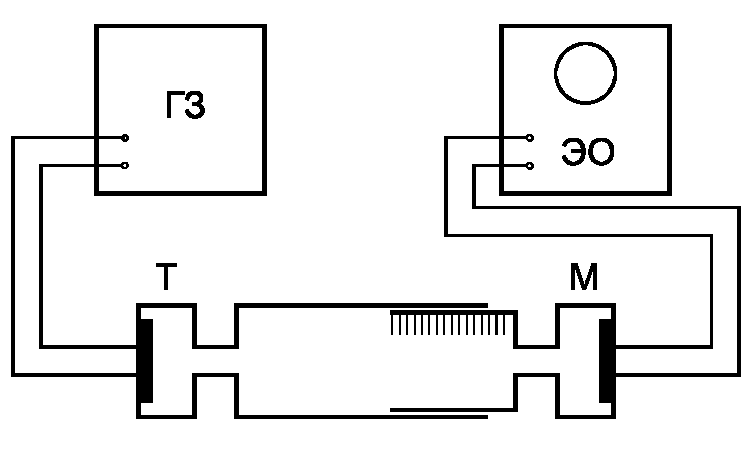
\includegraphics[width=0.7\linewidth]{ust}
	\caption{Установка для измерения скорости звука при помощи раздвижной трубы}
	\label{Fig:ust}
\end{center}
\end{figure}
\section{Обработка результатов измерений}
$L = (0.700\pm0.005)$ м --- начальная длина трубы, $T=(297.5\pm0.1)$ К --- температура в комнате. Табличные значения скоростей звука при данной температуре: $v_{\text{зв}}^{\text{возд}}=345.5\text{ м/с}$ и $v_{\text{зв}}^{\text{co}_2}=270.4\text{ м/с}$.

\subsection{Измерения при переменной длине трубы}
Найдём, при каких смещениях $x_k$ от начальной длины трубы происходит резонанс при данной частоте. Эксперимент проведём на увеличение и уменьшение длины трубы для воздуха и только на уменьшение для CO$_2$. Полученные данные занесём в таблицы \ref{tab:um_vozd}, \ref{tab:uv_vozd}, \ref{tab:uv_co2}. 
\begin{table}[h!]
	\centering
	\caption{Уменьшение трубы: воздух}
	\label{tab:um_vozd}
\begin{tabular}{|c|c|c|c|c|}
	\hline 
	& $x_1$, м & $x_2$ & $x_3$ & $x_4$ \\ 
	\hline 
	\rule[0ex]{0pt}{2.5ex} $f_1=(1.72\pm0.01)$ кГц & $(0.217\pm0.001)$ & $(0.118\pm0.001)$ & $(0.015\pm0.001)$ &  \\ 
	\hline 
	\rule[0ex]{0pt}{2.5ex} $f_2=(2.50\pm0.01)$ кГц & $(0.198\pm0.001)$ & $(0.129\pm0.001)$ & $(0.062\pm0.001)$ &  \\ 
	\hline 
	\rule[0ex]{0pt}{2.5ex} $f_3=(3.00\pm0.01)$ кГц & $(0.227\pm0.001)$ & $(0.169\pm0.001)$ & $(0.112\pm0.001)$ & $(0.053\pm0.001)$ \\ 
	\hline 
	\rule[0ex]{0pt}{2.5ex} $f_4=(4.00\pm0.01)$ кГц & $(0.168\pm0.001)$ & $(0.122\pm0.001)$ & $(0.081\pm0.001)$ & $(0.043\pm0.001)$ \\ 
	\hline 
\end{tabular} 
\end{table}

\begin{table}[h!]
	\centering
	\caption{Увеличение трубы: воздух}
	\label{tab:uv_vozd}
	\begin{tabular}{|c|c|c|c|c|}
		\hline 
		& $x_1$, м & $x_2$ & $x_3$ & $x_4$ \\ 
		\hline 
		\rule[0ex]{0pt}{2.5ex} $f_1=(1.72\pm0.01)$ кГц & $(0.016\pm0.001)$ & $(0.119\pm0.001)$ & $(0.218\pm0.001)$ &  \\ 
		\hline 
		\rule[0ex]{0pt}{2.5ex} $f_2=(2.50\pm0.01)$ кГц & $(0.061\pm0.001)$ & $(0.130\pm0.001)$ & $(0.199\pm0.001)$ &  \\ 
		\hline 
		\rule[0ex]{0pt}{2.5ex} $f_3=(3.00\pm0.01)$ кГц & $(0.053\pm0.001)$ & $(0.111\pm0.001)$ & $(0.170\pm0.001)$ & $(0.228\pm0.001)$ \\ 
		\hline 
		\rule[0ex]{0pt}{2.5ex} $f_4=(4.00\pm0.01)$ кГц & $(0.046\pm0.001)$ & $(0.082\pm0.001)$ & $(0.120\pm0.001)$ & $(0.169\pm0.001)$ \\ 
		\hline 
		\end{tabular} 
\end{table}

\begin{table}[h!]
	\centering
	\caption{Уменьшение трубы: CO$_2$}
	\label{tab:uv_co2}
	\begin{tabular}{|c|c|c|c|}
		\hline 
		& $x_1$, м & $x_2$, м & $x_3$, м\\ 
		\hline 
		\rule[0ex]{0pt}{2.5ex} $f_1=(1.70\pm0.01)$ кГц & $(0.174\pm0.001)$ & $(0.096\pm0.001)$ & $(0.017\pm0.001)$ \\ 
		\hline 
		\rule[0ex]{0pt}{2.5ex} $f_2=(2.03\pm0.01)$ кГц & $(0.228\pm0.001)$ & $(0.162\pm0.001)$ & $(0.097\pm0.001)$\\ 
		\hline 
		\rule[0ex]{0pt}{2.5ex} $f_3=(3.06\pm0.01)$ кГц & $(0.227\pm0.001)$ & $(0.185\pm0.001)$ & $(0.141\pm0.001)$\\ 
		\hline 
		\rule[0ex]{0pt}{2.5ex} $f_4=(4.05\pm0.01)$ кГц & $(0.217\pm0.001)$ & $(0.182\pm0.001)$ & $(0.155\pm0.001)$\\ 
		\hline
	\end{tabular}
	\begin{tabular}{|c|c|c|c|}
		\hline 
		$x_4$, м & $x_5$, м & $x_6$, м & $x_7$, м \\ 
		\hline 
		  &  &  &  \\ 
		\hline 
		\rule[0ex]{0pt}{2.5ex} $(0.003\pm0.001)$ &  &  &  \\ 
		\hline 
		\rule[0ex]{0pt}{2.5ex} $(0.097\pm0.001)$ & $(0.053\pm0.001)$ & $(0.008\pm0.001)$ &  \\ 
		\hline 
		\rule[0ex]{0pt}{2.5ex} $(0.122\pm0.001)$ & $(0.088\pm0.001)$ & $(0.055\pm0.001)$ & $(0.021\pm0.001)$ \\ 
		\hline 
	\end{tabular} 
\end{table}

Нанесём на график экспериментальные точки $x(k)$ и проведём по ним прямую методом наименьших квадратов (МНК, рис. \ref{fig:umvozd}, \ref{fig:uvvozd}, \ref{fig:um_co2}). Тогда $\lambda/2$ есть модуль углового коэффициента графика $x(k)$.
\begin{figure}
	\centering
	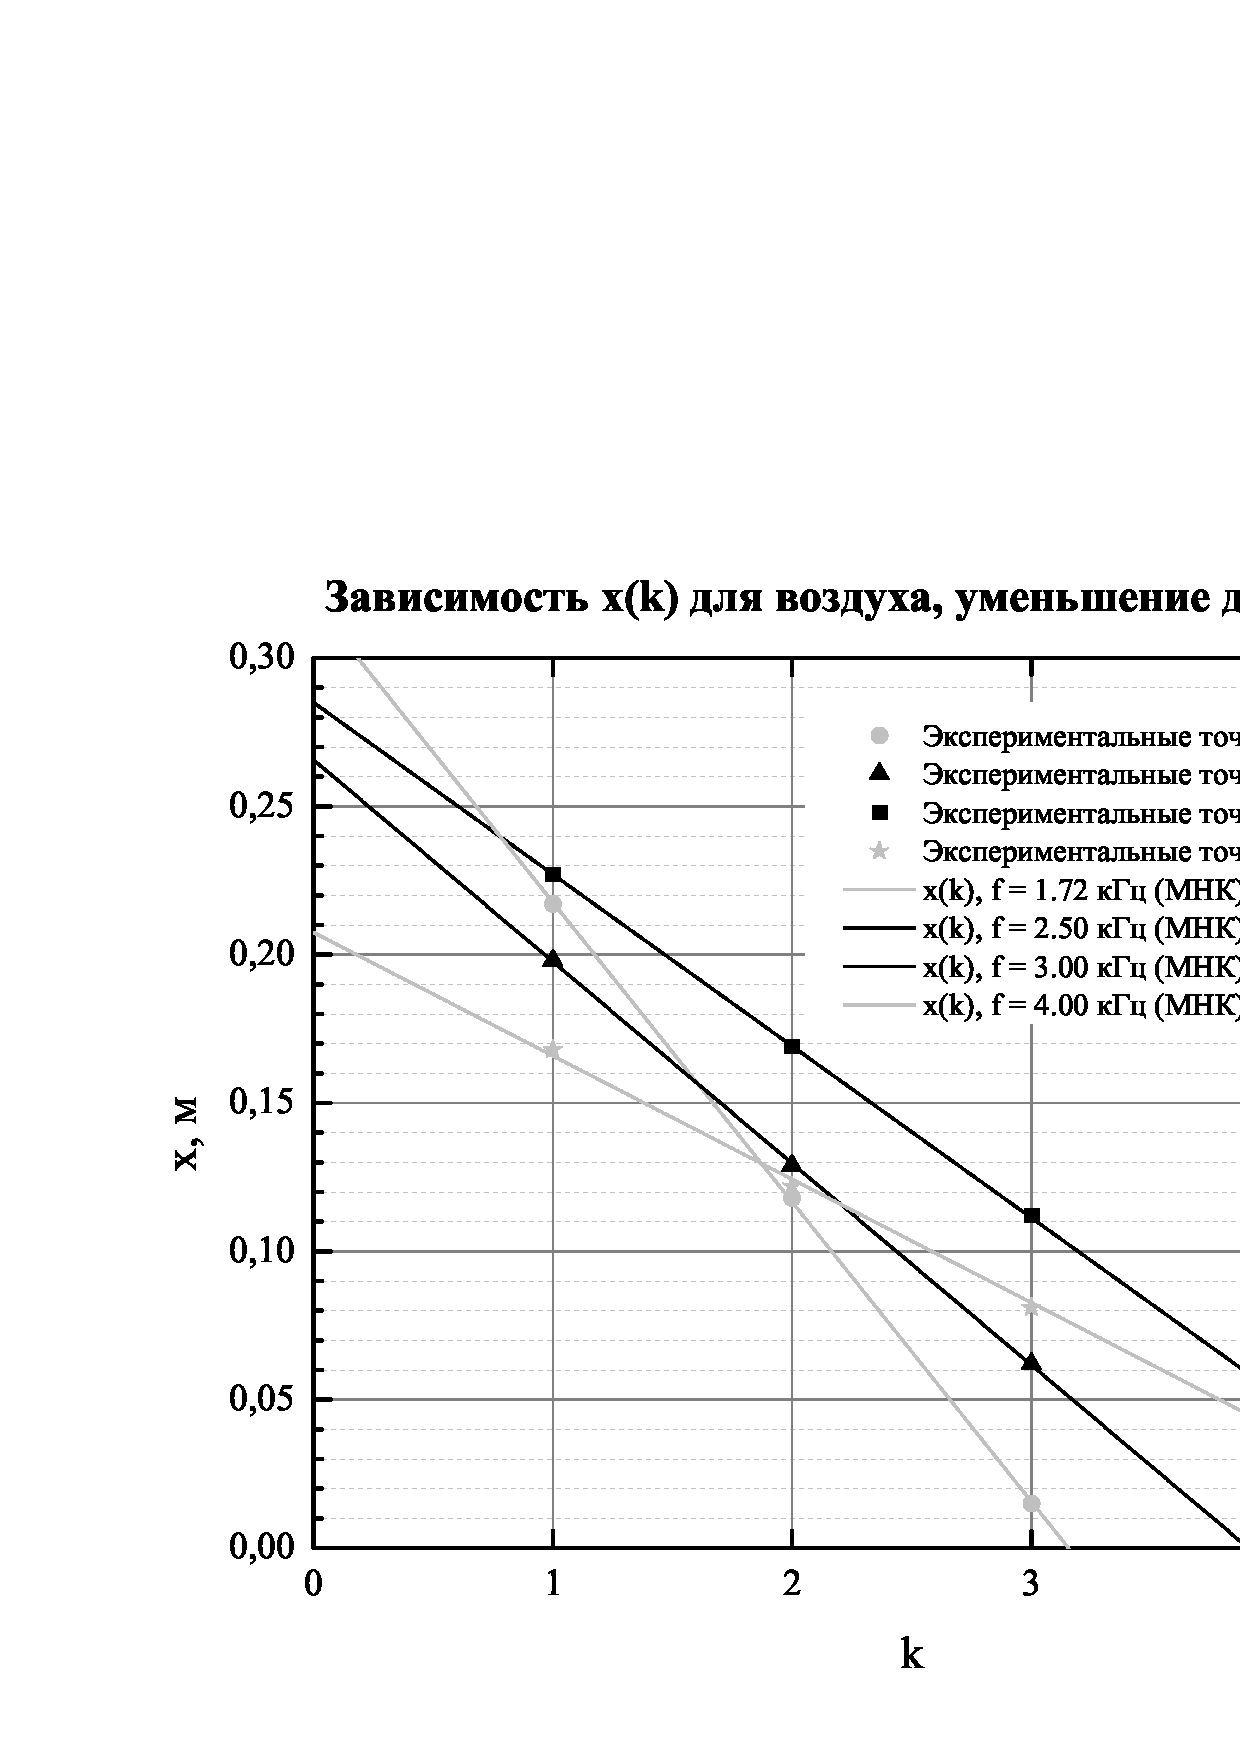
\includegraphics[width=0.8\linewidth]{um_vozd}
	\caption{Зависимость $x(k)$ для воздуха на уменьшение длины трубы}
	\label{fig:umvozd}
\end{figure}

\begin{figure}
	\centering
	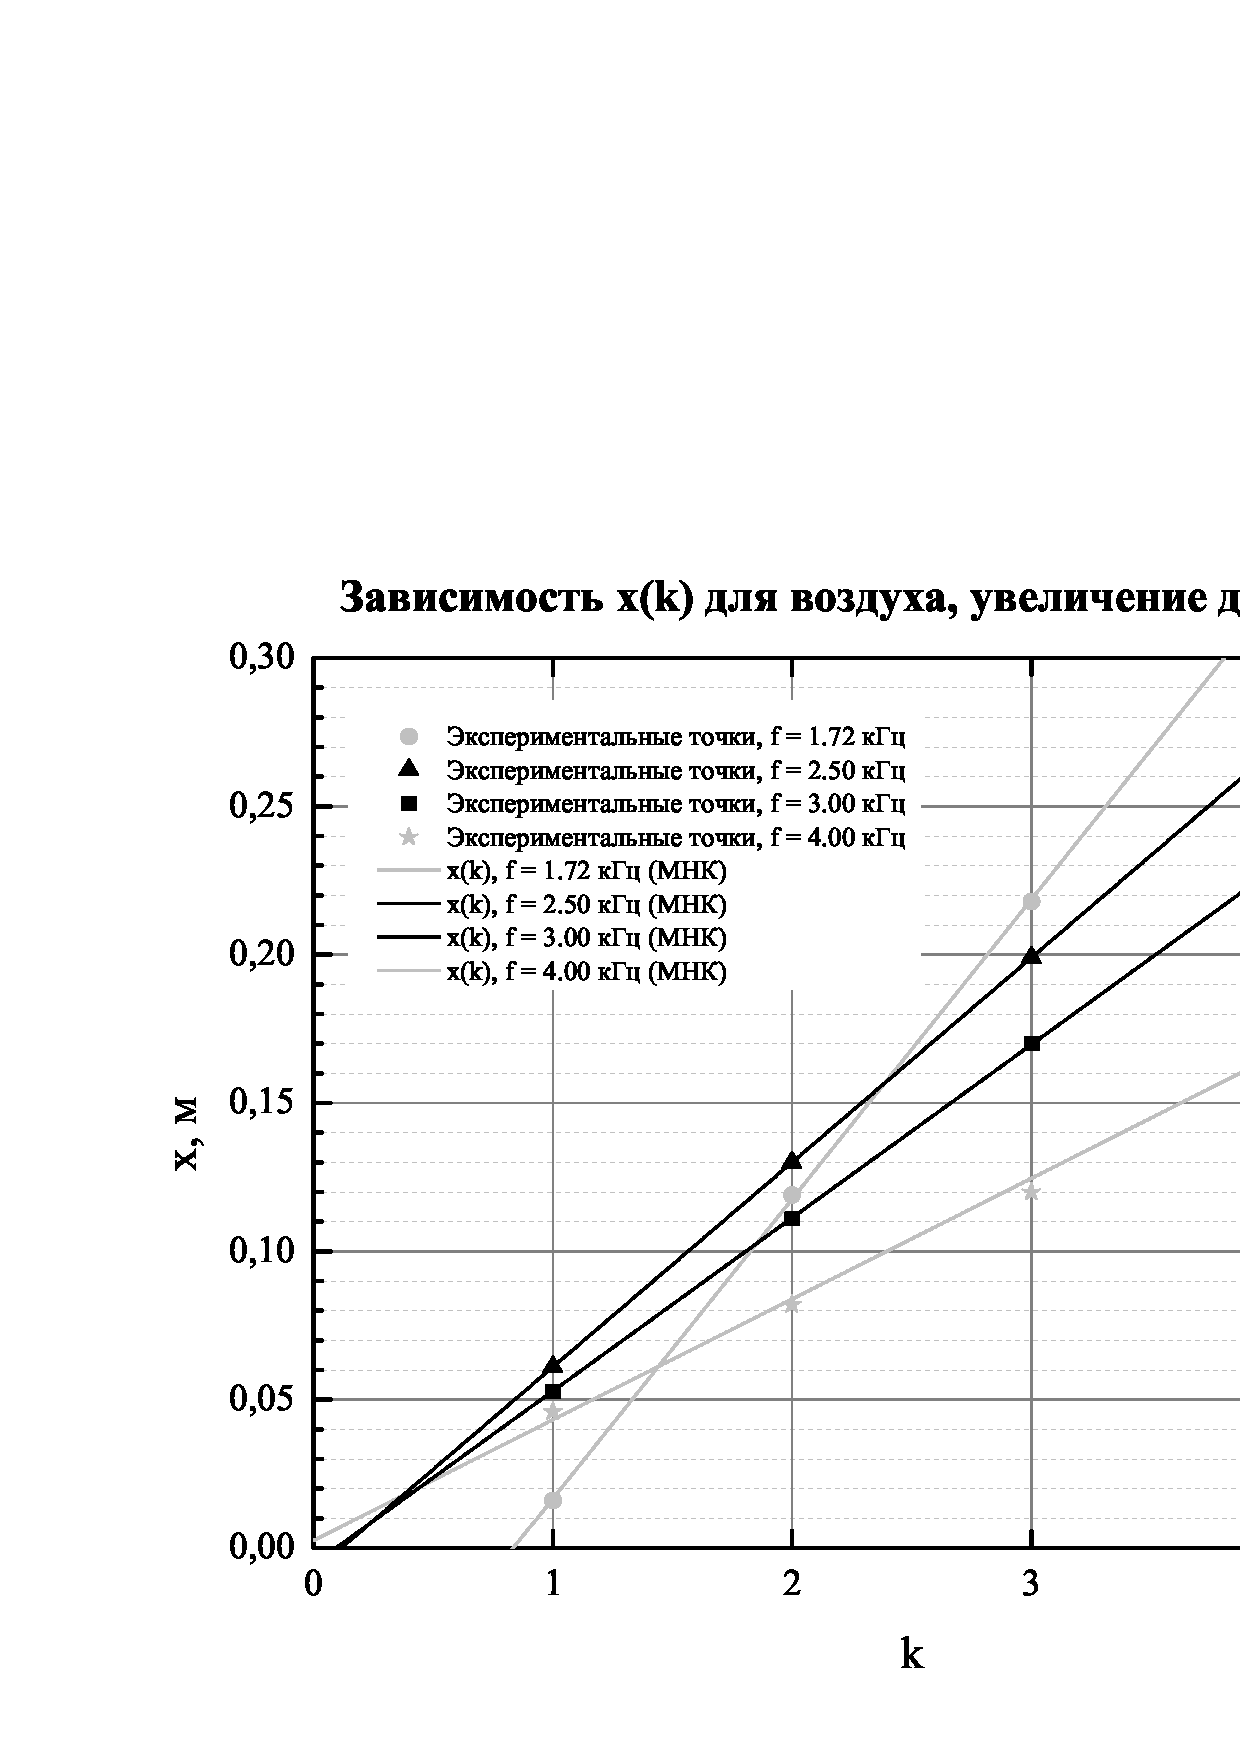
\includegraphics[width=0.8\linewidth]{uv_vozd}
	\caption{Зависимость $x(k)$ для воздуха на увеличение длины трубы}
	\label{fig:uvvozd}
\end{figure}

\begin{figure}
	\centering
	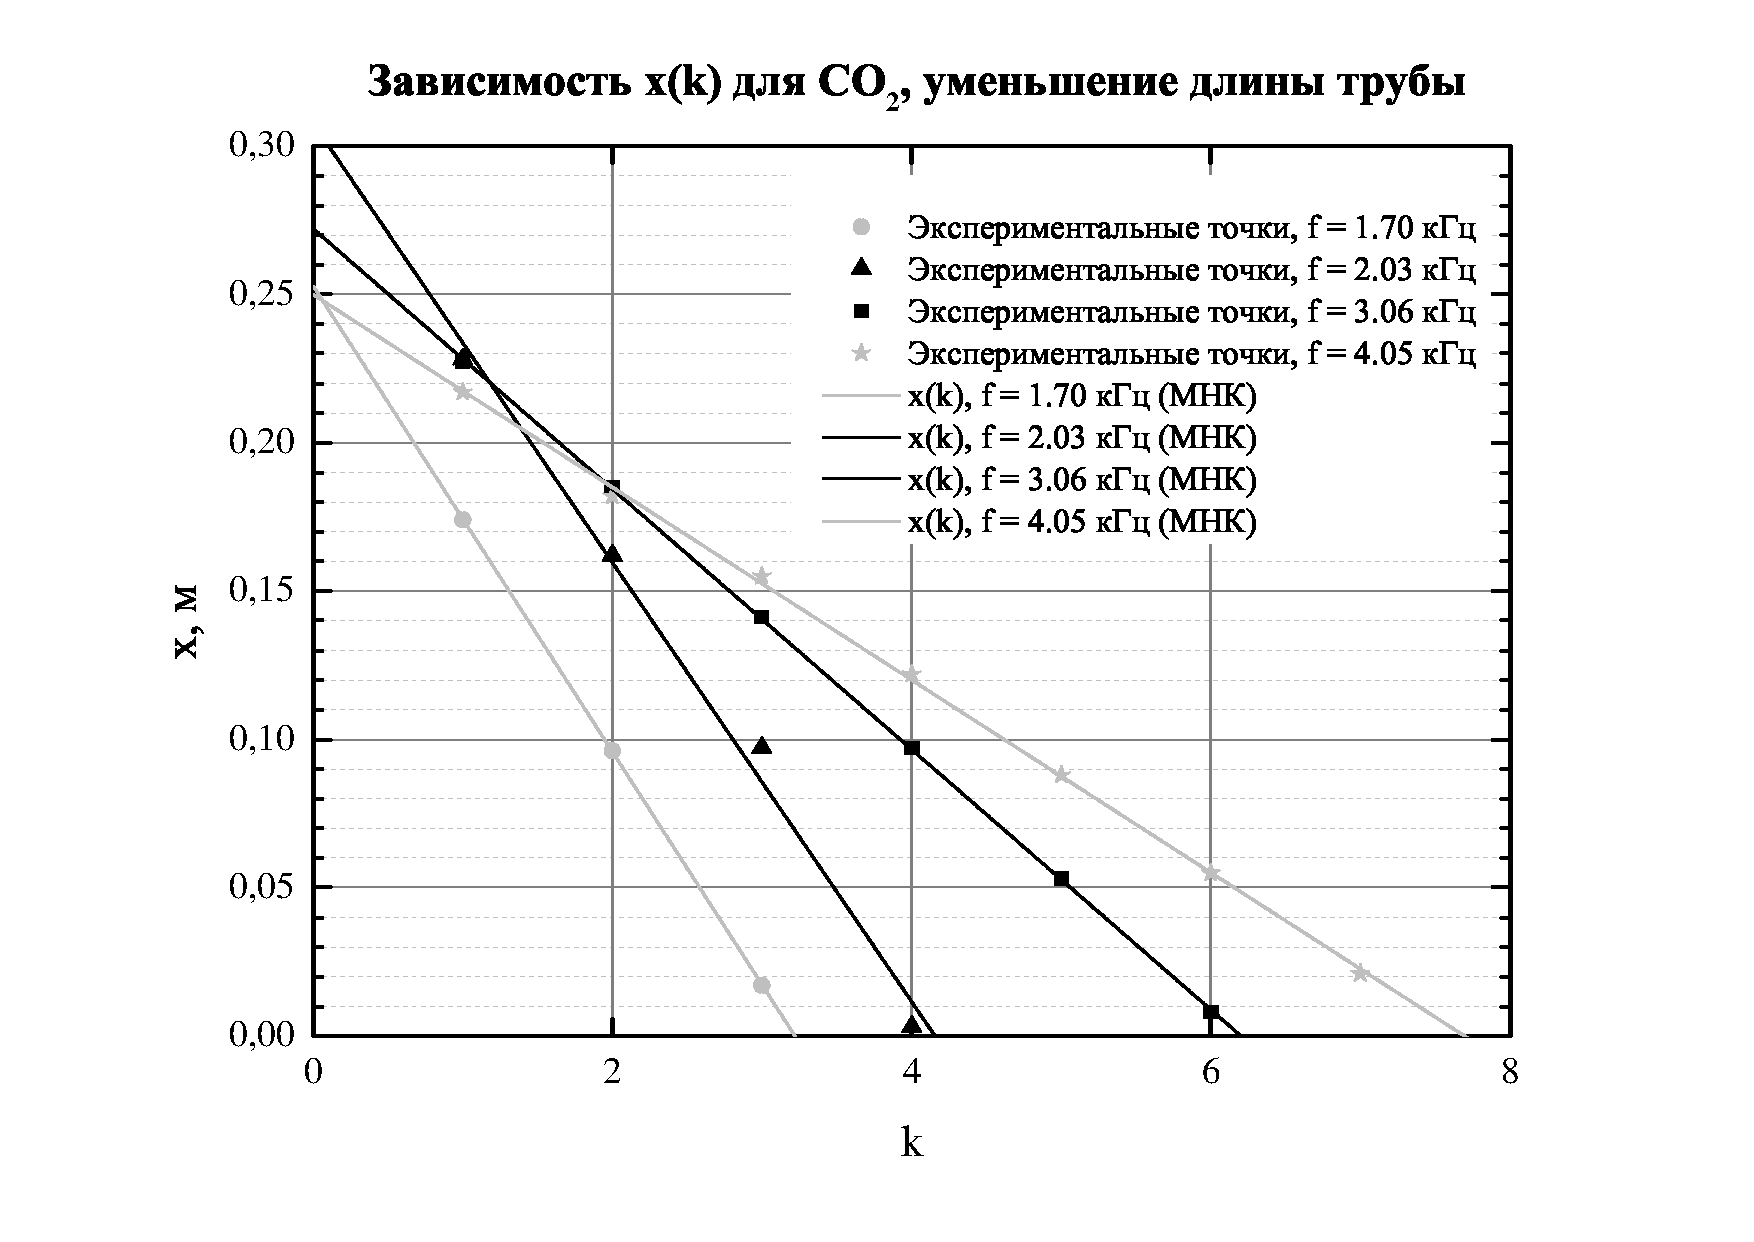
\includegraphics[width=0.8\linewidth]{um_co2}
	\caption{Зависимость $x(k)$ для CO$_2$ на уменьшение длины трубы}
	\label{fig:um_co2}
\end{figure}

Из МНК, получим результаты и занесём их в таблицы \ref{tab:resalt_vozd_um}, \ref{tab:resalt_vozd_uv}, \ref{tab:resalt_CO2_um}. 

\begin{table}[h]
	\centering
	\caption{Значения $\lambda /2$, воздух, уменьшение длины трубы}
	\label{tab:resalt_vozd_um}
\begin{tabular}{|c|c|}
	\hline 
	$f$, кГц & $\lambda /2$, м \\ 
	\hline 
	$(1.72\pm0.01)$ & $(0.1010\pm0.0012)$ \\ 
	\hline 
	$(2.50\pm0.01)$ & $(0.0680\pm0.0006)$ \\ 
	\hline 
	$(3.00\pm0.01)$ & $(0.0579\pm0.0003)$ \\ 
	\hline 
	$(4.00\pm0.01)$ & $(0.0416\pm0.0012)$ \\ 
	\hline 
\end{tabular} 
\end{table}

\begin{table}[h!]
	\centering
	\caption{Значения $\lambda /2$, воздух, увеличение длины трубы}
	\label{tab:resalt_vozd_uv}
	\begin{tabular}{|c|c|}
		\hline 
		$f$, кГц & $\lambda /2$, м \\ 
		\hline 
		$(1.72\pm0.01)$ & $(0.1010\pm0.0012)$ \\ 
		\hline 
		$(2.50\pm0.01)$ & $0.069$ \\ 
		\hline 
		$(3.00\pm0.01)$ & $(0.05840\pm0.00014)$ \\ 
		\hline 
		$(4.00\pm0.01)$ & $(0.041\pm0.002)$ \\ 
		\hline 
	\end{tabular} 
\end{table}

В таблице \ref{tab:resalt_vozd_uv} для частоты $f=(2.50\pm0.01)$ кГц погрешность для $\lambda /2$ из МНК получилась ровно 0 м.

\begin{table}[h!]
	\centering
	\caption{Значения $\lambda /2$, CO$_2$, уменьшение длины трубы}
	\label{tab:resalt_CO2_um}
	\begin{tabular}{|c|c|}
		\hline 
		$f$, кГц & $\lambda /2$, м \\ 
		\hline 
		$(1.70\pm0.01)$ & $(0.0785\pm0.0003)$ \\ 
		\hline 
		$(2.03\pm0.01)$ & $(0.074\pm0.005)$ \\ 
		\hline 
		$(3.06\pm0.01)$ & $(0.0439\pm0.0002)$ \\ 
		\hline 
		$(4.05\pm0.01)$ & $(0.0326\pm0.0004)$ \\ 
		\hline 
	\end{tabular} 
\end{table}

Теперь для каждого случая найдём скорость звука в данной среде по формуле
$$
v_{\text{зв}}=2 \cdot \lambda/2 \cdot f,
$$
а погрешность по формуле:
$$
\pogk{v_{\text{зв}}}=\pogk{\lambda} + \pogk{f},
$$
и результаты занесём в таблицы \ref{tab:resalt_v_vozd_um}, \ref{tab:resalt_v_vozd_uv}, \ref{tab:resalt_v_CO2_um}.
\begin{table}[h!]
	\centering
	\caption{Значения $v_{\text{зв}}$, воздух, уменьшение длины трубы}
	\label{tab:resalt_v_vozd_um}
	\begin{tabular}{|c|c|}
		\hline 
		$f$, кГц & $v_{\text{зв}}$, м/c \\ 
		\hline 
		$(1.72\pm0.01)$ & $(347\pm5)$ \\ 
		\hline 
		$(2.50\pm0.01)$ & $(340\pm3)$ \\ 
		\hline 
		$(3.00\pm0.01)$ & $(347\pm2)$ \\ 
		\hline 
		$(4.00\pm0.01)$ & $(333\pm10)$ \\ 
		\hline 
	\end{tabular} 
\end{table}

\begin{table}[h!]
	\centering
	\caption{Значения $v_{\text{зв}}$, воздух, увеличение длины трубы}
	\label{tab:resalt_v_vozd_uv}
	\begin{tabular}{|c|c|}
		\hline 
		$f$, кГц & $v_{\text{зв}}$, м/с \\ 
		\hline 
		$(1.72\pm0.01)$ & $(347\pm5)$ \\ 
		\hline 
		$(2.50\pm0.01)$ & $(345\pm1)$ \\ 
		\hline 
		$(3.00\pm0.01)$ & $(350\pm1)$ \\ 
		\hline 
		$(4.00\pm0.01)$ & $(326\pm16)$ \\ 
		\hline 
	\end{tabular} 
\end{table}

\begin{table}[h!]
	\centering
	\caption{Значения $v_{\text{зв}}$, CO$_2$, уменьшение длины трубы}
	\label{tab:resalt_v_CO2_um}
	\begin{tabular}{|c|c|}
		\hline 
		$f$, кГц & $v_{\text{зв}}$, м/с \\ 
		\hline 
		$(1.70\pm0.01)$ & $(267\pm2)$ \\ 
		\hline 
		$(2.03\pm0.01)$ & $(300\pm20)$ \\ 
		\hline 
		$(3.06\pm0.01)$ & $(268\pm2)$ \\ 
		\hline 
		$(4.05\pm0.01)$ & $(263\pm3)$ \\ 
		\hline 
	\end{tabular} 
\end{table}
\vspace{2cm}
Таким образом, самыми близкими к табличном значениям скорости звука оказались результаты:
\begin{center}
$f = (3.00\pm0.01)$ кГц, $v_{\text{зв}}^{\text{возд ум}} = (347\pm2)$ м/с\\
$f = (2.50\pm0.01)$ кГц, $v_{\text{зв}}^{\text{возд ув}} = (345\pm1)$ м/с\\
$f = (3.06\pm0.01)$ кГц, $v_{\text{зв}}^{\text{co$_2$ ум}} = (268\pm2)$ м/с\\
\end{center}

Найдём по формуле \eqref{Eq:gamma} показатель адиабаты $\gamma$ для воздуха и углекислого газа. Погрешность вычислим так:
\begin{equation}
\pogk{\gamma}=\pogk{T}+4\pogk{v_{\text{зв}}}.
\label{Eq:pog_gamma}
\end{equation}
Для воздуха $\mu_{\text{возд}} = 0.02898$ кг/моль, а для CO$_2$ $\mu_{\text{co$_2$}} = 0.04401$ кг/моль, $R = 8.314$ Дж/(моль~$\cdot$~К).

Получим такие результаты:
\begin{table}[h!]
	\centering
	\caption{Значения $\gamma$}
	\label{tab:gamma_res}
	\begin{tabular}{|c|c|c|}
		\hline 
		Условие&$v_{\text{зв}}$, м/с & $\gamma$\\ 
		\hline 
		Воздух, ум.&$(347\pm2)$ & $(1.411\pm0.016)$ \\ 
		\hline 
		Воздух, ув.&$(345\pm1)$ & $(1.394\pm0.008)$ \\ 
		\hline 
		CO$_2$, ум.&$(268\pm2)$ & $(1.278\pm0.019)$ \\ 
		\hline 
	\end{tabular} 
\end{table}

Значения находятся в хорошем согласии с табличными данными ($\gamma_{\text{возд}}=1.40,\ \gamma_{\text{co$_2$}}=1.30$).
\subsection{Измерения при постоянной длине трубы}

Также будем искать резонансные частоты при фиксированной длине трубы $L$ для воздуха и CO$_2$. Данные занесём в таблицы \ref{tab:rez_v}, \ref{tab:rez_ug}.

\begin{table}[h!]
	\centering
	\caption{Резонансные частоты при длине трубы $L$: воздух}
	\label{tab:rez_v}
	\begin{tabular}{|c|c|}
		\hline 
		\rule[0ex]{0pt}{2.5ex} $f_1$, кГц & --- \\ 
		\hline 
		\rule[0ex]{0pt}{2.5ex} $f_2$, кГц & $(0.477\pm0.001)$ \\ 
		\hline 
		\rule[0ex]{0pt}{2.5ex} $f_3$, кГц & $(0.760\pm0.001)$ \\ 
		\hline 
		\rule[0ex]{0pt}{2.5ex} $f_4$, кГц & $(0.937\pm0.001)$ \\ 
		\hline 
		\rule[0ex]{0pt}{2.5ex} $f_5$, кГц & $(1.24\pm0.01)$ \\ 
		\hline 
		\rule[0ex]{0pt}{2.5ex} $f_6$, кГц & $(1.41\pm0.01)$ \\ 
		\hline 
	\end{tabular} 
\end{table}

\begin{table}[h!]
	\centering
	\caption{Резонансные частоты при длине трубы $L$: CO$_2$}
	\label{tab:rez_ug}
	\begin{tabular}{|c|c|}
		\hline 
		\rule[0ex]{0pt}{2.5ex} $f_1$, кГц & --- \\ 
		\hline 
		\rule[0ex]{0pt}{2.5ex} $f_2$, кГц & $(0.395\pm0.001)$ \\ 
		\hline 
		\rule[0ex]{0pt}{2.5ex} $f_3$, кГц & $(0.614\pm0.001)$ \\ 
		\hline 
		\rule[0ex]{0pt}{2.5ex} $f_4$, кГц & $(0.755\pm0.001)$ \\ 
		\hline 
		\rule[0ex]{0pt}{2.5ex} $f_5$, кГц & $(0.998\pm0.001)$ \\ 
		\hline 
		\rule[0ex]{0pt}{2.5ex} $f_6$, кГц & $(1.14\pm0.01)$ \\ 
		\hline 
	\end{tabular} 
\end{table}
Нанесём на график экспериментальные точки $f(k)$ и проведём по ним прямую методом наименьших квадратов (МНК, через начало координат, рис. \ref{fig:fiks_len}). Тогда $\frac{v_{\text{зв}}}{2L}$ есть модуль углового коэффициента графика $f(k)$.

\begin{figure}[h!]
	\centering
	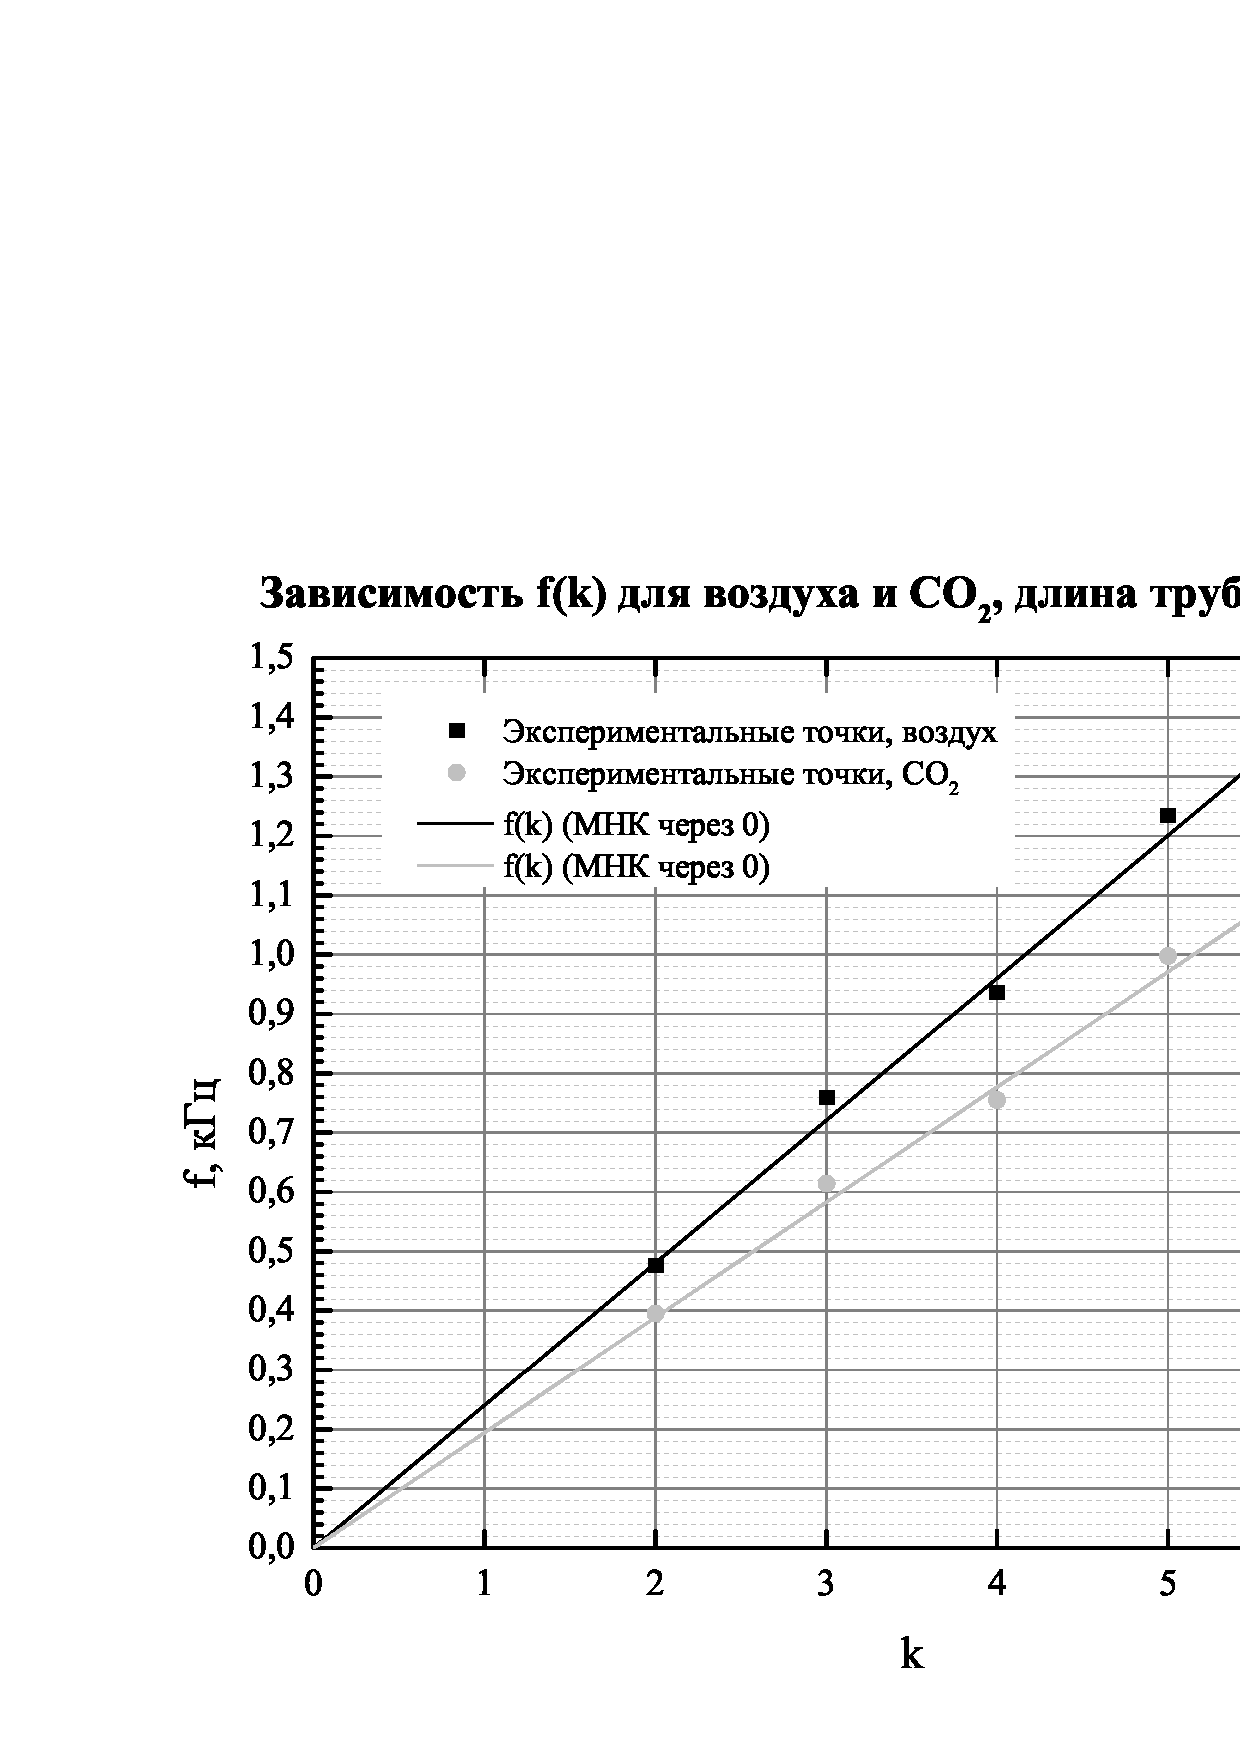
\includegraphics[width=0.8\linewidth]{fiks_len}
	\caption{Зависимость $f(k)$ для воздуха и CO$_2$, длина трубы фиксирована и равна $L$}
	\label{fig:fiks_len}
\end{figure}

Из МНК имеем:
$$
\cfrac{v_{\text{зв}}^{\text{возд}}}{2L} = (0.240\pm0.003)\cdot 10^3\text{ с$^{-1}$}\\
$$
$$
\cfrac{v_{\text{зв}}^{\text{co$_2$}}}{2L} = (0.194\pm0.003)\cdot 10^3\text{ с$^{-1}$}
$$
Отсюда найдём скорости звука:
$$
v_{\text{зв}}^{\text{возд}} = (336\pm5)\text{ м/с}
$$
$$
v_{\text{зв}}^{\text{co$_2$}} = (272\pm4)\text{ м/с}
$$
По формулам \eqref{Eq:gamma} и \eqref{Eq:pog_gamma} найдём значение $\gamma$:
$$
\gamma_{\text{возд}}=(1.323\pm0.039)
$$
$$
\gamma_{\text{co$_2$}}=(1.316\pm0.039)
$$

Видим, что значения скорости звука в воздухе и $\gamma_{\text{возд}}$ не совпадают с табличными значениями, а значение скорости звука в угл. газе и значение показателя адиабаты находятся в достаточном согласовании с табличными значениями.

\section{Заключение}
В данной работе мы исследовали резонанс газа в трубе и появление стоячих волн.

Определив длины трубы, при которых происходит резонанс, на определённых частотах нашли длину волны. Отсюда получили значения показателя адиабаты $\gamma$ в 3 случаях: $\gamma_{\text{возд}}^{\text{ум}}=(1.411\pm0.016),\ \gamma_{\text{возд}}^{\text{ув}}=(1.394\pm0.008),\ \gamma_{\text{co$_2$}}^{\text{ум}}=(1.278\pm0.019)$, которые находятся в достаточном согласием с табличными данными.

Также определили скорость звука при фиксированной длине трубы, откуда нашли значения показателя адиабаты: $\gamma_{\text{возд}}=(1.323\pm0.039),\ \gamma_{\text{co$_2$}}=(1.316\pm0.039)$.
\bibliography{mybibliography}
\bibliographystyle{gost705}

\end{document}
